\chapter{Evaluation}
\label{chap:eval}

In this chapter, we present the evaluation results of the RUMIS system. We focus on testing the quality of rule revisions in terms of the conviction measure, as well the prediction quality. The chapter is organized as follows. First, the setting of the experiment is discussed. Second, the quality of rulesets and the facts they predict are assessed. Finally, we present the runtime performance of the system RUMIS on different real-world datasets.

\section{Setting}

\textbf{Dataset.} To measure the quality of rules and their predictions, the ideal graph $\cG^i$, i.e. the KG containing all true facts about the real world, is required. However, constructing $\cG^i$ is obviously not possible. Hence, instead we treat the given graph as an approximation of the ideal KG $\cG^i_{\mi{appr}}$. To obtain the available (training) KG $\cG^a$ we remove from $\cG^i_{\mi{appr}}$ 20\% of the facts for every binary relation, and retain all unary facts in $\cG^i_{\mi{appr}}$. It is guaranteed that there is no isolated vertex in $\cG^a$, i.e the node which is not connected to any other nodes in the graph. In our experiment, YAGO3~\cite{ref28}, Wikidata Football and IMDB~\footnote{\url{http://people.mpi-inf.mpg.de/~gadelrab/downloads/ILP2016}} datasets are used as the ideal KGs. YAGO3 covers a variety of domains and contains roughly 1.8 million entities, 38 predicates, and 20.7 million triples. Meanwhile, IMDB only focus on movie content collected from the IMDB website~\footnote{\url{http://imdb.com}}, there are 112 thousand entities, 38 predicates and 583 thousand triples in this KG. Besides, to construct the Wikidata Football for our experiments, we sample 1 million facts with 238 thousand entities and 443 predicates from football domain of the original Wikidata KG~\footnote{\url{https://www.wikidata.org}}. %In details, thanks to randomly choosing facts in the format \textit{$<$subject$>$ $<$memberOf$>$ $<$object$>$} where \textit{$<$object$>$} is in the list of manually chosen popular football clubs, famous footballers and coaches (seeding set) are sampled from Wikidata. After that, all the entities that can be visited from any node in the seeding set (chosen entities) by following paths (one or more consecutive links/edges/predicates in the original Wikidata KG) are collected for the ideal KG. These chosen entities and all possible links between them in the original Wikidata KG are sampled for the smaller scale. This new KG is expected to have specific domain where facts are related to football and sports.

Figure~\ref{fig:venn} depicts the ideal, approximated and available KGs as well the extended KGs $\cG_{\cR_{\mi{H}}}$, $\cG_{\cR_{\mi{NM}}}$ obtained by resp. applying $\cR_H$ and its revision $\cR_{NM}$ to $\cG^a$. The RUMIS system aims to tackle the KG completion problem by narrowing the difference between the $\cG_{\cR_{\mi{NM}}}$ and $ \cG^i$.

\begin{figure}[ht]
\centering
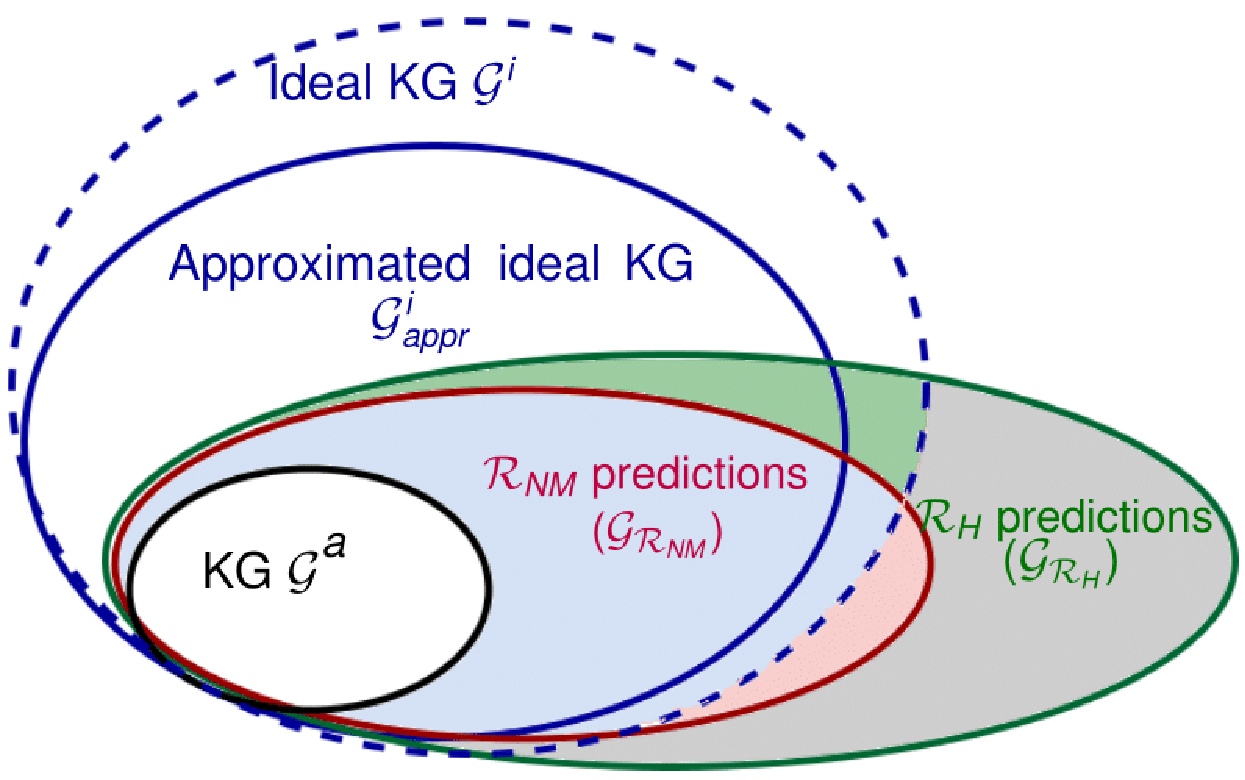
\includegraphics[width=0.55\textwidth]{figures/big_pic_exp}
\caption{The Ideal, Available and Extended KGs.}
\label{fig:venn}
\end{figure}

\textbf{Experimental Setup.} In our experiments, RUMIS is executed on a server which has Linux OS, 40 cores and 400GB RAM memory. As the data preparation, positive rules in the format \textit{h(X, Z) $\leftarrow$ p(X, Y), q(Y, Z)} are extracted from $\cG^a$ and ranked according to the \textit{absolute support} measure. The positive rule mining function of RUMIS (see Chapter~\ref{chap:system}) is exploited in this step. After that, the positive rules are revised following the approach presented in Chapter~\ref{chap:frame}. The \textit{conviction} measure is used as the $\mi{rm}$ rule measure. Various exception ranking earlier described strategies are realized in RUMIS. The resulting rule revisions are stored in $\mi{\cR_{N}}$, $\mi{\cR_{PM}}$ and $\mi{\cR_{OPM}}$, resp.

\section{Ruleset Quality}

We present the evaluation results of the rule quality assessment in Table~\ref{tab:rules_quality1} and~\ref{tab:rules_quality2} for YAGO, IMDB and Wikidata Football, resp. For every row in the tables, we fix the top-$\mi{k}$ ($k=5,30,$ ... $100$) positive rules $\cR_{H}$ that will be subsequently revised. Then the \textit{average conviction} of the rules and their revisions are found for YAGO, IMDB and Wikidata Football by using RUMIS. Naturally the quality of the revised rules is better than that of their positive versions w.r.t. conviction. Besides, in general while the average quality of every column has a decreasing trend with the appearance of rules having lower precision levels, the enhancement ratio between positive rules and their revisions increases and reaches the peak of $7.8\%$ and $10.3\%$ for top-100 IMDB and top-30 Wikidata Football rules, resp. The results show that the introduction of negated atoms significantly boost up the rule precision.

\begin{table}[ht]
\centering
\footnotesize
\renewcommand*{\arraystretch}{1.07}
\centering



%\footnotesize{
%\resizebox{\columnwidth}{!}{%
%
%\begin{tabular}{|l|llll|llll|llll|}
%\hline
%       \multirow{2}{*}{\textbf{\textit{topk}}}                    & \multicolumn{4}{c|}{\textbf{YAGO}}        & \multicolumn{4}{c|}{\textbf{IMDB}}  & \multicolumn{4}{c|}{\textbf{Sample WIKIDATA}}      \\ \cline{2-13} 
%       %\hline
% & $\cR_{H}$ & $\cR_{N}$ & $\cR_{PM}$ & $\cR_{OPM}$ & $\cR_{H}$ & $\cR_{N}$ & $\cR_{PM}$ & $\cR_{OPM}$ & $\cR_{H}$ & $\cR_{N}$ & $\cR_{PM}$ & $\cR_{OPM}$ \\ \hline
%5   & 1.3784 & 1.3821 & 1.3821 & 1.3821 & 2.2670 & 2.3014 & 2.3008 & 2.3014 & 3.2282 & 3.2342 & 3.2340 & 3.2342\\ %\hline
%30   & 1.1207 & 1.1253 & 1.1236 & 1.1237 & 1.5453 & 1.5644 & 1.5543 & 1.5640 & 3.1118 & 3.4315 & 3.4194 & \textbf{3.4271}\\ %\hline
%50   & 1.0884 & 1.0923 & 1.0909 & 1.0913 & 1.3571 & 1.3749 & 1.3666 & 1.3746  & 2.7115 & 2.9193 & 2.9070 & 2.9135\\ %\hline
%60   & 1.0797 & 1.0837 & 1.0823 & 1.0829 & 1.3063 & 1.3221 & 1.3143 & 1.3219  & 2.4930 & 2.7101 & 2.6986 & 2.7046\\ %\hline
%70   & 1.0714 & 1.0755 & 1.0736 & 1.0744 & 1.2675 & 1.2817 & 1.2746 & 1.2814  & 2.3395 & 2.5272 & 2.3931 & 2.5219\\ %\hline
%80   & 1.0685 & 1.0731 & 1.0710 & 1.0720 & 1.2368 & 1.2499 & 1.2431 & 1.2497  & 2.4071 & 2.5781 & 2.4597 & 2.5734\\ %\hline
%100   & 1.0618 & 1.0668 & 1.0648 & 1.0659 & 1.3074 & 1.4100 & 1.3987 & 1.4098  & 2.3258 & 2.4847 & 2.3859 & 2.4806\\ \hline
%
%\end{tabular}
%
%}
%}

\begin{tabular}{|l|llll|llll|}
\hline
       \multirow{2}{*}{\textbf{\textit{topk}}}                    & \multicolumn{4}{c|}{\textbf{YAGO}}        & \multicolumn{4}{c|}{\textbf{IMDB}}      \\ \cline{2-9} 
       %\hline
 & $\cR_{H}$ & $\cR_{N}$ & $\cR_{PM}$ & $\cR_{OPM}$ & $\cR_{H}$ & $\cR_{N}$ & $\cR_{PM}$ & $\cR_{OPM}$ \\ \hline
5   & 1.3784 & 1.3821 & 1.3821 & 1.3821 & 2.2670 & 2.3014 & 2.3008 & 2.3014\\ %\hline
30   & 1.1207 & 1.1253 & 1.1236 & 1.1237 & 1.5453 & 1.5644 & 1.5543 & 1.5640\\ %\hline
50   & 1.0884 & 1.0923 & 1.0909 & 1.0913 & 1.3571 & 1.3749 & 1.3666 & 1.3746\\ %\hline
60   & 1.0797 & 1.0837 & 1.0823 & 1.0829 & 1.3063 & 1.3221 & 1.3143 & 1.3219\\ %\hline
70   & 1.0714 & 1.0755 & 1.0736 & 1.0744 & 1.2675 & 1.2817 & 1.2746 & 1.2814\\ %\hline
80   & 1.0685 & 1.0731 & 1.0710 & 1.0720 & 1.2368 & 1.2499 & 1.2431 & 1.2497\\ %\hline
100   & 1.0618 & 1.0668 & 1.0648 & 1.0659 & 1.3074 & 1.4100 & 1.3987 & 1.4098\\ \hline

\end{tabular}

% \centering
% \caption{My caption}
% \label{my-label}
% \begin{tabular}{l|l|l|l|l|l|l|l|l|}
% \cline{2-9}
%                            & \multicolumn{4}{c|}{YAGO manual}        & \multicolumn{4}{c|}{IMDB top rules}        \\ \hline
% \multicolumn{1}{|l|}{\textit{topk}} & $\cR_{H}$ & $\cR_{N}$ & $\cR_{PM}$ & $\cR_{OPM}$ & $\cR_{H}$ & $\cR_{N}$ & $\cR_{PM}$ & $\cR_{OPM}$ \\ \hline
% \multicolumn{1}{|l|}{5}    &   1.10    &   1.11    &    1.20    &    1.15     &   2.27    &   2.3    &   2.89     &  2.55       \\ \hline
% \multicolumn{1}{|l|}{10}   &    1.10   &   1.11    &    1.23    &    1.18     &   1.9    &   1.92    &    4.74    &  2.07       \\ \hline
% \multicolumn{1}{|l|}{15}   &   1.12    &   1.13    &    1.32    &    1.18     &   1.8    &   1.82    &   5.25     &   1.98      \\ \hline
% \multicolumn{1}{|l|}{20}   &       &       &        &         &       &       &        &         \\ \hline
% \end{tabular}

\smallskip
\caption{The Average Quality of the Top Positive and Nonmonotonic Rules for YAGO, IMDB.}
\label{tab:rules_quality1}
%\vspace*{-1.7\baselineskip}
\end{table}

\begin{table}[ht]
\centering
\footnotesize
\renewcommand*{\arraystretch}{1.07}
\centering



%\footnotesize{
%\resizebox{\columnwidth}{!}{%
%
%\begin{tabular}{|l|llll|llll|llll|}
%\hline
%       \multirow{2}{*}{\textbf{\textit{topk}}}                    & \multicolumn{4}{c|}{\textbf{YAGO}}        & \multicolumn{4}{c|}{\textbf{IMDB}}  & \multicolumn{4}{c|}{\textbf{Sample WIKIDATA}}      \\ \cline{2-13} 
%       %\hline
% & $\cR_{H}$ & $\cR_{N}$ & $\cR_{PM}$ & $\cR_{OPM}$ & $\cR_{H}$ & $\cR_{N}$ & $\cR_{PM}$ & $\cR_{OPM}$ & $\cR_{H}$ & $\cR_{N}$ & $\cR_{PM}$ & $\cR_{OPM}$ \\ \hline
%5   & 1.3784 & 1.3821 & 1.3821 & 1.3821 & 2.2670 & 2.3014 & 2.3008 & 2.3014 & 3.2282 & 3.2342 & 3.2340 & 3.2342\\ %\hline
%30   & 1.1207 & 1.1253 & 1.1236 & 1.1237 & 1.5453 & 1.5644 & 1.5543 & 1.5640 & 3.1118 & 3.4315 & 3.4194 & \textbf{3.4271}\\ %\hline
%50   & 1.0884 & 1.0923 & 1.0909 & 1.0913 & 1.3571 & 1.3749 & 1.3666 & 1.3746  & 2.7115 & 2.9193 & 2.9070 & 2.9135\\ %\hline
%60   & 1.0797 & 1.0837 & 1.0823 & 1.0829 & 1.3063 & 1.3221 & 1.3143 & 1.3219  & 2.4930 & 2.7101 & 2.6986 & 2.7046\\ %\hline
%70   & 1.0714 & 1.0755 & 1.0736 & 1.0744 & 1.2675 & 1.2817 & 1.2746 & 1.2814  & 2.3395 & 2.5272 & 2.3931 & 2.5219\\ %\hline
%80   & 1.0685 & 1.0731 & 1.0710 & 1.0720 & 1.2368 & 1.2499 & 1.2431 & 1.2497  & 2.4071 & 2.5781 & 2.4597 & 2.5734\\ %\hline
%100   & 1.0618 & 1.0668 & 1.0648 & 1.0659 & 1.3074 & 1.4100 & 1.3987 & 1.4098  & 2.3258 & 2.4847 & 2.3859 & 2.4806\\ \hline
%
%\end{tabular}
%
%}
%}

\begin{tabular}{|l|llll|}
\hline
       \multirow{2}{*}{\textbf{\textit{topk}}}          & \multicolumn{4}{c|}{\textbf{WIKIDATA Football}}      \\ \cline{2-5} 
       %\hline
 & $\cR_{H}$ & $\cR_{N}$ & $\cR_{PM}$ & $\cR_{OPM}$ \\ \hline
5  & 3.2282 & 3.2342 & 3.2340 & 3.2342\\ %\hline
30   & 3.1118 & 3.4315 & 3.4194 & \textbf{3.4271}\\ %\hline
50   & 2.7115 & 2.9193 & 2.9070 & 2.9135\\ %\hline
60   & 2.4930 & 2.7101 & 2.6986 & 2.7046\\ %\hline
70   & 2.3395 & 2.5272 & 2.3931 & 2.5219\\ %\hline
80   & 2.4071 & 2.5781 & 2.4597 & 2.5734\\ %\hline
100   & 2.3258 & 2.4847 & 2.3859 & 2.4806\\ \hline

\end{tabular}

% \centering
% \caption{My caption}
% \label{my-label}
% \begin{tabular}{l|l|l|l|l|l|l|l|l|}
% \cline{2-9}
%                            & \multicolumn{4}{c|}{YAGO manual}        & \multicolumn{4}{c|}{IMDB top rules}        \\ \hline
% \multicolumn{1}{|l|}{\textit{topk}} & $\cR_{H}$ & $\cR_{N}$ & $\cR_{PM}$ & $\cR_{OPM}$ & $\cR_{H}$ & $\cR_{N}$ & $\cR_{PM}$ & $\cR_{OPM}$ \\ \hline
% \multicolumn{1}{|l|}{5}    &   1.10    &   1.11    &    1.20    &    1.15     &   2.27    &   2.3    &   2.89     &  2.55       \\ \hline
% \multicolumn{1}{|l|}{10}   &    1.10   &   1.11    &    1.23    &    1.18     &   1.9    &   1.92    &    4.74    &  2.07       \\ \hline
% \multicolumn{1}{|l|}{15}   &   1.12    &   1.13    &    1.32    &    1.18     &   1.8    &   1.82    &   5.25     &   1.98      \\ \hline
% \multicolumn{1}{|l|}{20}   &       &       &        &         &       &       &        &         \\ \hline
% \end{tabular}

\smallskip
\caption{The Average Quality of the Top Positive and Nonmonotonic Rules for Wikidata Football.}
\label{tab:rules_quality2}
%\vspace*{-1.7\baselineskip}
\end{table}

The enhancement ratio between revisions of the three ranking methods and the top positive rules is shown in Figure~\ref{fig_1_5_imdb}, ~\ref{fig_1_5_yago} and ~\ref{fig_1_5_wikidata} for IMDB, YAGO and Wikidata Football, resp. In these figures, the height and the width are corresponding to the top-$k$ and the improvement rate of the average conviction. One can observe that the rate has an uptrend, in general the more low quality Horn rules are added to the top ruleset, the higher is the improvement rate. The Naive ranking shows the best results w.r.t. the rule quality, which is obviously expected.

With IMDB dataset, the results of Naive and OPM ranking are approximately the same and slightly better than PM ranking. For the top-100 rules, the best average improvement of 7.8\% is achieved. It can be seen that the quality of positive rules around top-100 are much worse than the rest, resulting in the sharp increase between top-80 and top-100 in the Figure~\ref{fig_1_5_imdb}.

\begin{figure}[ht]
\centering
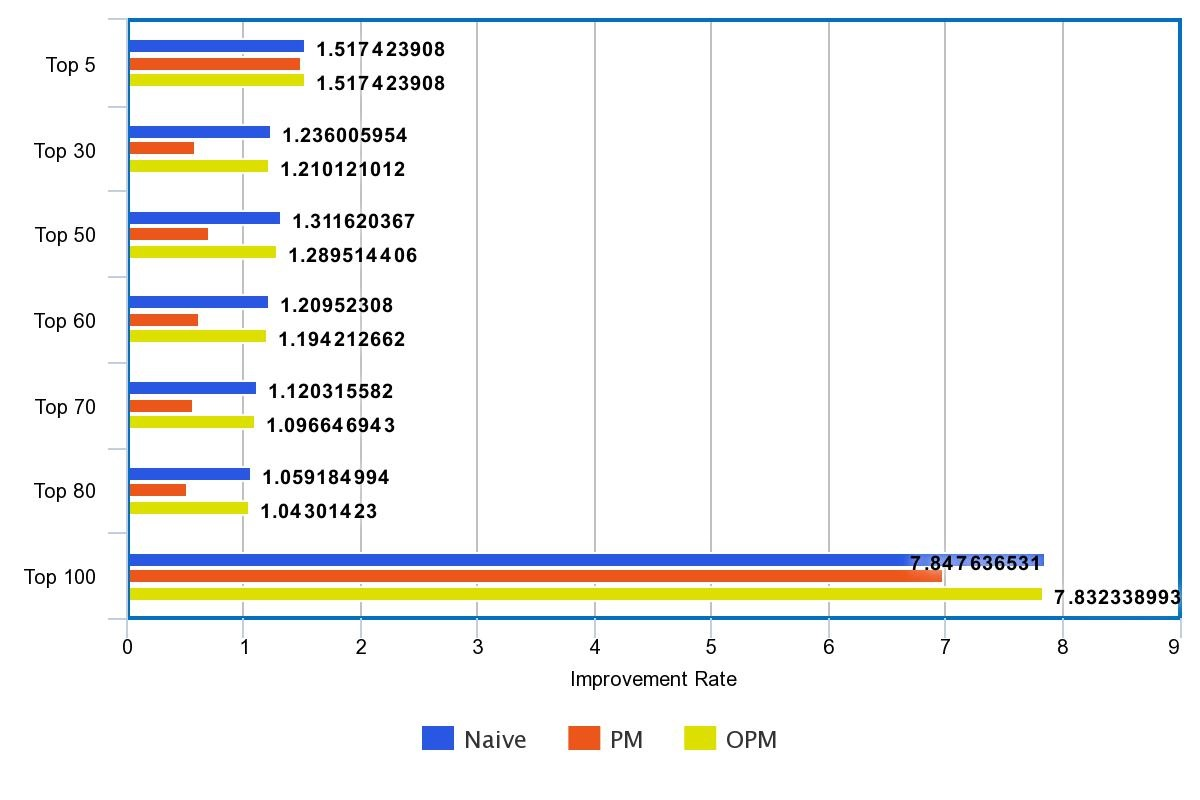
\includegraphics[width=0.85\textwidth]{figures/table_1_5_imdb.jpeg}
\caption{The Average Conviction Improvement Rate (\%) of Rules Revised using Our Methods and IMDB Dataset.}
\label{fig_1_5_imdb}
\end{figure}

Figure~\ref{fig_1_5_yago} shows that in general the improvement rates for the average conviction in YAGO increase. However, the contrast between the highest and the lowest in this figure is not as large as in IMDB data due to the qualities of top-100 Horn rules in YAGO are not highly different.

\begin{figure}[ht]
\centering
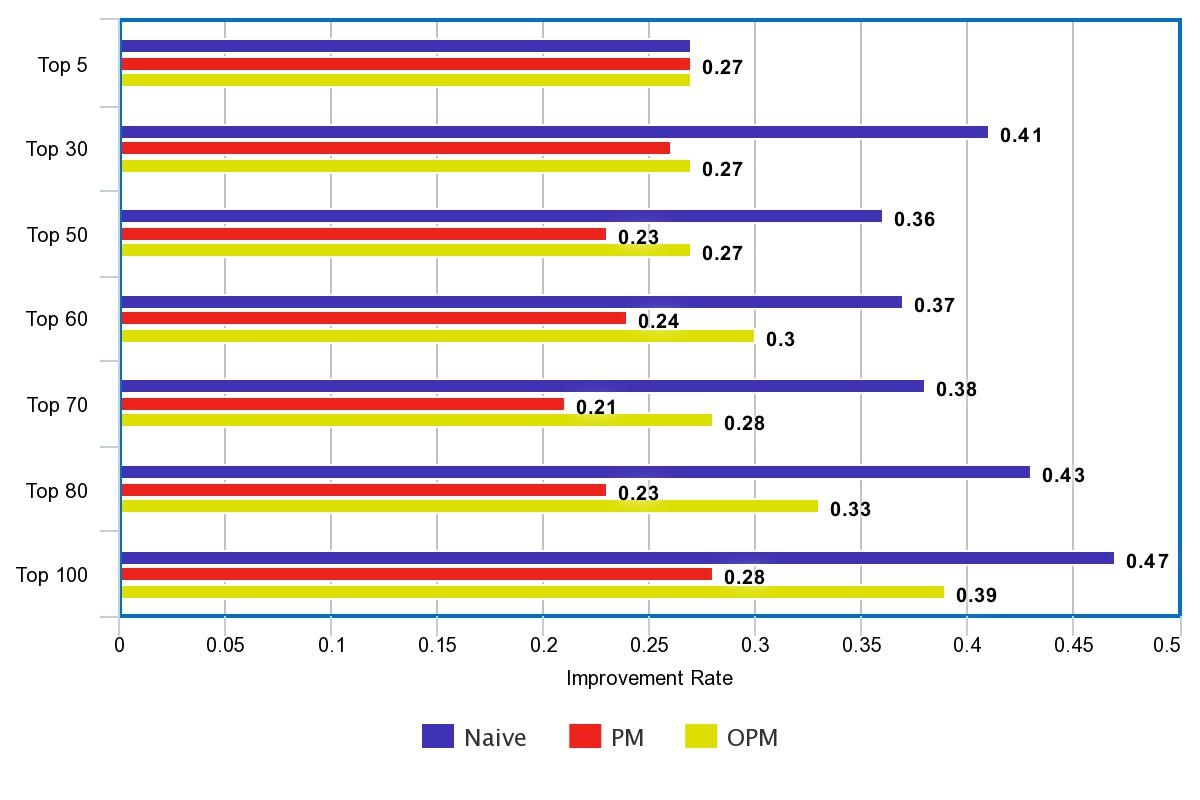
\includegraphics[width=0.85\textwidth]{figures/table_1_5_yago.jpeg}
\caption{The Average Conviction Improvement Rate (\%) of Rules Revised using Our Methods and YAGO Dataset.}
\label{fig_1_5_yago}
\end{figure}

As regards the Wikidata Football, Figure~\ref{fig_1_5_wikidata} witnesses an interesting pattern where the improvement rate significantly climbs from top-5 to top-30. It can be seen that RUMIS mines very good exceptions for positive rules around top-30, 
resulting in a peak of more than 10\% enhancement ratio for this dataset.

\begin{figure}[ht]
\centering
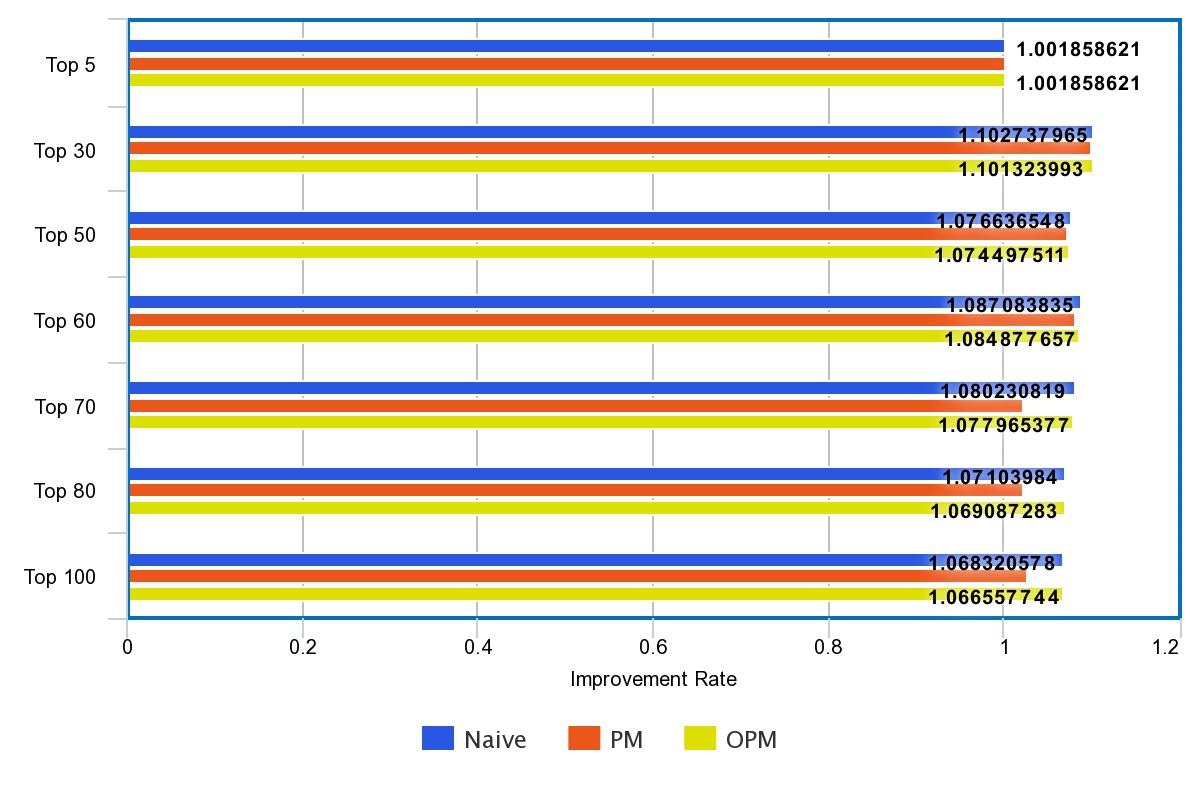
\includegraphics[width=0.85\textwidth]{figures/table_1_5_wikidata.jpeg}
\caption{The Average Conviction Improvement Rate (\%) of Rules Revised using Our Methods and Wikidata Football Dataset.}
\label{fig_1_5_wikidata}
\end{figure}

\section{Prediction Quality}

We now describe the evaluation procedure for estimating the predictive quality of the revised rules. Among top-50 (for IMDB, YAGO3) and top-300 (for Wikidata Football) positive rules mined from the KG, 5 are sampled as $\cR_H$ and then the revision procedure is applied for these rules. After that, the predictions of the rules from $\cR_H$ and their revisions are analyzed to evaluate our approaches.

To this end, these rulesets are applied to the learning KG $\cG^a$ and the corresponding predicted facts are generated by DLV tool~\cite{dlv}. Subsequently, we achieve $\cG_{\cR_\mi{H}}$, $\cG_{\cR_\mi{N}}$, $\cG_{\cR_\mi{PM}}$ and $\cG_{\cR_\mi{OPM}}$ for $\cR_H$ and revisions of $\cR_H$, resp. The statistics is shown in Table~\ref{tab:prediction_res}, where the first three columns indicate the head relations of the rules in $\cR_H$, the number of new predictions, i.e. predicted facts not included in $\cG^a$ and the part of these predictions which are outside $\cG^i_{\mi{appr}}$, resp. The statistics in the second and third columns is available for positive rules and all of their revisions.

\begin{table}[ht]
\centering

% \begin{tabular}{c|l|llll|llll}
% \hline
%  \multirow{2}{*}{}              &   \multirow{2}{*}{\textbf{$\mi{head(r)}$}}   	& \multicolumn{4}{c|}{\textbf{predictions}} 						&  \multicolumn{4}{c}{\textbf{outside $\cG^i_{appr}$}}  				\\ \cline{3-10} 
%          						&  									& $\cR_\mi{H}$  & $\cR_{N}$ & $\cR_{PM}$  		& $\cR_{OPM}$ &  $\cR_\mi{H}$     & $\cR_{\mi{N}}$ 	& $\cR_\mi{PM}$     & $\cR_{\mi{OPM}}$    \\ \hline
% %\multirow{4}{*}{\rotatebox{90}{YAGO}}
% & directed & 41079 & 39174 & 39174 & 39174  & 41021 & 39116 & 39116 & 39116 \\ %\cline{2-10}
%  & gradFrom & 3519 & 3456 & 3456 & 3456  & 3363 & 3300 & 3300 & 3300 \\ %\cline{2-10}
%  & citizenOf & 3407 & 2883 & 2883 & 2883  & 3360 & 2836 & 2836 & 2836 \\ %\cline{2-10}
%  & bornIn & 110283 & 108317 & 109846 & 108317 & 109572 & 107607 & 109137 & 107607 \\ \hline\hline %\cline{1-10}
% %\multirow{4}{*}{\rotatebox{90}{IMDB}} 
% & actIn & 1231 & 1214 & 1230 & 1214 & 1148 & 1131 & 1147 & 1131 \\ %\cline{2-10}
%  & genre & 629 & 609 & 618 & 609  & 493 & 477 & 482 & 477 \\% \cline{2-10}
%  & hasLang & 173 & 102 & 125 & 102 & 163 & 92 & 115 & 92 \\ %\cline{2-10}
%  & prodIn & 2489 & 2256 & 2327 & 2327 & 2488 & 2255 & 2326 & 2326 \\ \cline{1-10}
% \end{tabular}
\footnotesize{
\resizebox{\columnwidth}{!}}}  				\\ \cline{2-12} 
 		& $\cR_\mi{H}$  & $\cR_{\mi{N}}$ & $\cR_{\mi{PM}}$  		& $\cR_{\mi{OPM}}$ &  $\cR_\mi{H}$     & $\cR_{\mi{N}}$ 	& $\cR_\mi{PM}$     & $\cR_{\mi{OPM}}$  & $\cR_{\mi{N}}$ 	& $\cR_\mi{PM}$     & $\cR_{\mi{OPM}}$   \\ \hline

%\multirow{4}{*}{\rotatebox{90}{IMDB}} 
 $\mi{{I}{:}{actedIn}}$ & 1231 & 1214 & 1230 & 1214 & 1148 & 1131 & 1147 & 1131 &90 & 100 & 90\\ %\cline{2-10}
 $\mi{{I}{:}{genre}}$ & 629 & 609 & 618 & 609  & 493 & 477 & 482 & 477 &50 & 20 & 50\\% \cline{2-10}
 $\mi{{I}{:}{hasLang}}$ & 173 & 102 & 125 & 102 & 163 & 92 & 115 & 92 &  60 & 100 & 60\\ %\cline{2-10}
 $\mi{{I}{:}{prodIn}}$ & 2489 & 2256 & 2327 & 2327 & 2488 & 2255 & 2326 & 2326 & 10 & 10 & 30 \\ \cline{10-12}
 &  &  &  &  &  &  &  &  	& 52.50  & 45.16   & \textbf{57.75}  \\
\hline 
$\mi{{Y}{:}{direct}}$ & 41079 & 39174 & 39174 & 39174  & 41021 & 39116 & 39116 & 39116 & 100 & 100 & 100   \\
 $\mi{{Y}{:}{grFrom}}$ & 3519 & 3456 & 3456 & 3456  & 3363 & 3300 & 3300 & 3300 & 100 & 100 & 70 \\ 
 $\mi{{Y}{:}{citizOf}}$ & 3407 & 2883 & 2883 & 2883  & 3360 & 2836 & 2836 & 2836 & 50 & 50 & 70 \\ 
 $\mi{{Y}{:}{bornIn}}$ & 110283 & 108317 & 109846 & 108317 & 109572 & 107607 & 109137 & 107607 &90& 90 & 100 \\ \cline{10-12}  
 &  &  &  &  &  &  &  &  	& 85  & 85   & 85 \\
 \hline 
 \end{tabular}}}

\smallskip
\caption{New Facts Predicted by the Rulesets for IMDB (\textit{I}), YAGO (\textit{Y}) and Wikidata Football (\textit{W}).}
\label{tab:prediction_res}
%\vspace*{-1.7\baselineskip}
\end{table}

One can see that not many predicted facts are included in $\cG^i_{\mi{appr}}$ ($\approx$9\% for IMDB and $\approx$2\% for YAGO ideal KGs). This can be explained by the fact that YAGO is a highly incomplete general purpose KG. Moreover, it is crucial to note that the sampled Horn rules and their revisions generate approximately the same number of correctly predicted facts which are present in $\cG^i_{\mi{appr}}$. More specifically, in all three datasets $\cG_{\mi{\cR_H}}\backslash \cG_{\mi{\cR_{PM}}} \cap \cG^i_{\mi{appr}}=\emptyset$ means that the grey region has nothing in common with the approximated ideal KG in Figure~\ref{fig:venn}, in other words, the addition of exceptions does not lead to the removal of correct predictions from $\cG^i_{\mi{appr}}$.

To guarantee the fairness of the comparison between predictions generated by different rulesets, it is necessary to keep the $\cR_H$ not totally incorrect. Indeed, provided that the sampled positive rules always generate inaccurate facts, inserting arbitrary negated atoms may filter out some incorrect predictions, resulting in the rule enhancement, yet the rules themselves would still be of poor quality. Furthermore, observe that the number of predictions made by $\cR_H$ outside $\cG^i_{\mi{appr}}$ (third column of Table~\ref{tab:prediction_res}) is rather large. To verify these predictions, unfortunately no ground truth is available. Thus, we have to manually check the generated facts using the Internet resource. Since the number of the facts to be checked is huge, we propose to randomly select maximum 20 new predictions for each head predicate in $\cR_H$ and verify them. For the IMDB, YAGO and Wikidata Football, 70\%, 30\% and 55\% of predictions respectively turned out to be indeed correct. This shows that the quality of the positive rules that we start with is acceptable.

Since the size of the set difference between predictions made by $\cR_H$ and extended by applying $\cR_H$ and its revisions is also huge, we have to proceed further with sampling to evaluate the predictive quality of the revision. Here for each head relation from the set differences $\cG_{\cR_\mi{H}}\backslash \cG_{\cR_{\mi{N}}}$, $\cG_{\cR_\mi{H}}\backslash \cG_{\cR_{\mi{PM}}}$ and $\cG_{\cR_\mi{H}}\backslash \cG_{\cR_{\mi{OPM}}}$, maximum 10 facts have been randomly sampled for manual check. In the last column of the Table~\ref{tab:prediction_res}, the proportion of incorrect facts in the difference sets are presented. These facts are called ``correctly removed", since they correspond to false prediction made by $\cR_H$ but avoided by the respective revisions (the grey region in in Figure~\ref{fig:venn}). For the IMDB dataset, among all the revision strategies, OPM ranking always performs best with 57.75\% and 97.5\% correctly removed predictions for IMDB and Wikidata Football, resp. Meanwhile, all the rankers demonstrate the same results (85\%) for the YAGO KG. Since the predictive power of the positive rules in IMDB is better than those in YAGO, the revision of the latter makes a more visible impact than the former.

\section{Running Times}

In our experiment, top-100 positive rules are mined from IMDB and YAGO while this number of Wikidata Football is 300. Table~\ref{tab:run_time} provides statistics about running times (in seconds) of three different steps in the RUMIS system. More specifically, the second row of this table indicates how long for mining Horn rules and exception witness sets. In addition, the third and fourth rows present the average running times (over three ranking methods Naive, PM, OPM) of resp. ranking exceptions and extending KGs with DLV.

\begin{table}[ht]
\centering
\footnotesize{
\begin{tabular}{|c|ccc|}
\hline
\textbf{Steps} & \textbf{IMDB} & \textbf{YAGO} & \textbf{Wikidata Football}\\
\hline
 \textit{Horn Rule and EWS Mining} & 7 & 68 & 193\\
 \textit{Exception Ranking} & 32 & 111 & 2940\\
 \textit{Extension with DLV} & 8 & 310 & 180\\
 \hline 
\end{tabular}
}
\smallskip
\caption{Running Times for Each Step of the Three Datasets}
\label{tab:run_time}
%\vspace*{-1.7\baselineskip}
\end{table}

It can be seen that the numbers of Wikidata Football for the first two steps are the largest since the quantity of positive rules mined from this dataset is much bigger than that of IMDB or YAGO. Meanwhile, among the three datasets, YAGO has the most number of facts, resulting in the longest time to extend the KG using DLV (310 seconds).

\begin{figure}[t]
    \centering
   
    \vspace{-.2cm}
    \begin{tabular}{l}
 {\scriptsize
        $\mi{r_1: writtenBy(X, Z)}  \leftarrow
        \mi{hasPredecessor(X, Y)},\mi{writtenBy(Y, Z)},$ $ \textbf{not}$  $\mi{american\_film(X)} $}\\        
       {\scriptsize 
$\mi{r_2:  actedIn(X, Z)}  \leftarrow
        \mi{isMarriedTo(X, Y)},\mi{directed(Y, Z)},$ $ \textbf{not}$  $\mi{silent\_film\_actor(X)} $} \\
          {\scriptsize 
$\mi{r_3:  isPoliticianOf(X, Z)}  \leftarrow
        \mi{hasChild(X, Y)}{,}\mi{isPoliticianOf(Y, Z)}{,}$$ \textbf{not}$  $\mi{vicepresidentOfMexico(X)} $} \\
          {\scriptsize 
$\mi{r_4:  hasCitizenship(X, Z)}  \leftarrow
        \mi{hasFather(X, Y)}{,}\mi{hasCitizenship(Y, Z)}{,}$$ \textbf{not}$  $\mi{countryOfTheUK(Z)} $} \\
 \end{tabular}            
    \caption{Examples of the Revised Rules}
 \label{fig:examplerules}
 \vspace{-.4cm}
\end{figure}

\textbf{Example rules.} Some interesting examples are presented in the Figure~\ref{fig:examplerules}. Here 
the rule $\mi{r_1}$ mined from IMDB dataset indicates that normally movies in the same series are written by the same writer except the American movies. The rule $\mi{r_3}$ generated from YAGO reveals an interesting pattern from domain politics, i.e, typically fathers and sons are politicians in the same country unless the fathers are Mexican vice-presidents. Being mined from Wikidata Football, the rule $\mi{r_4}$ shows that father and son usually have the same citizenship, except the case that the father holds a citizenship in the UK (countries such as England, Northern Ireland, Wales and Scotland).